\subsection{Simulation}
For the simulation of the circuit has been used the same test-bench since the external entity of the circuit has not been modified with respect to the previous implementation.
In \autoref{fig:wave_start_j} the timing with the signals of the DUT is shown.In this case when the $VIN$ signal becomes valid 4 clock periods are required until the first result is available at the output; the explanation for this longer latency is due to the pipeline stages introduced in the circuit.

\begin{figure}[h]
	\center
	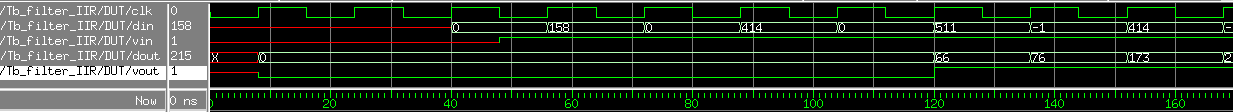
\includegraphics[width=1\textwidth]{wave_start_j_look_ahead.png}
	\caption{Start of the simulation}
	\label{fig:wave_start_j}
\end{figure}

Finally in \autoref{fig:wave_vin_j} it is observed the correct operation of the circuit when $VIN$ becomes low and then high. The internal registers do not sample when $VIN$ is not asserted, so the output data does not change, keeping the output valid. When $VIN$ returns to $1$, only one clock period is required before the output changes value because the registers are already full.

\begin{figure}[h]
	\center
	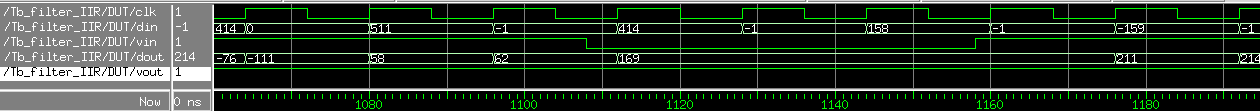
\includegraphics[width=1\textwidth]{wave_vin_0_1_j_look_ahead.png}
	\caption{Simulation of $VIN$ signal transition}
	\label{fig:wave_vin_j}
\end{figure}

Once the correct timing of the circuit has been verified, the output data has been compared with the corresponding C implementation of the realized model. With the same set of data used for the test-bench of the previous architecture, the same output results were obtained. You can refer to the data shown in \autoref{tab:tab_results} to have an outline of the results.